\section{Definition of the ultimate display}
\label{sec:definition}
\begin{figure}[h]
    \centering
    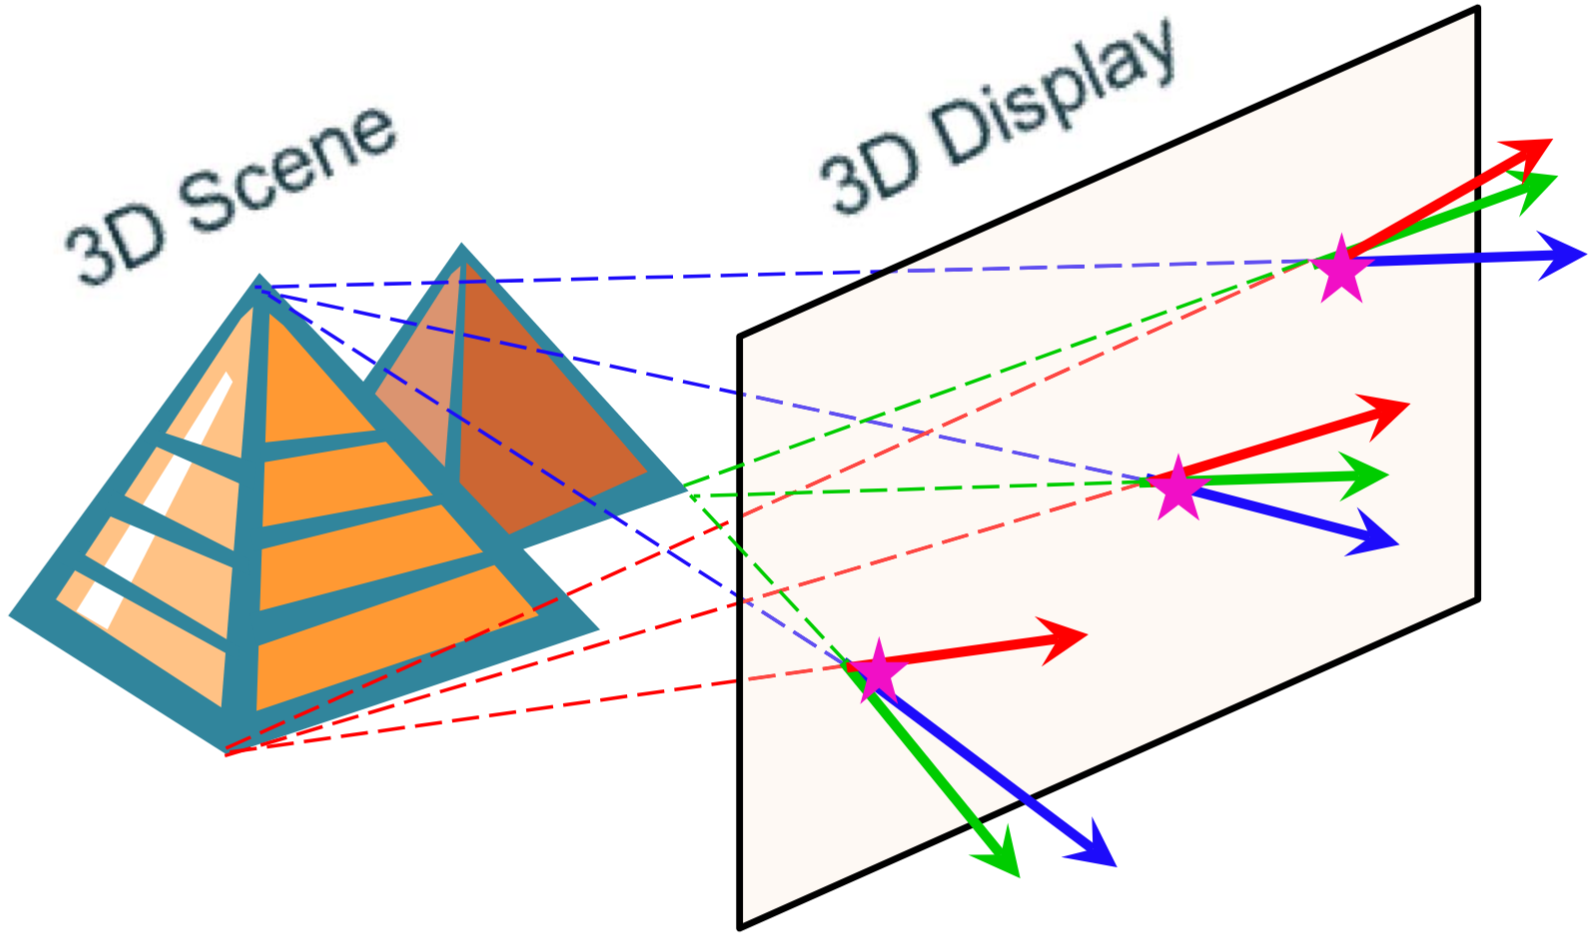
\includegraphics[width=\linewidth]{assets/window}
    \caption{The ultimate display reproduces the position, direction, wavelength, and amplitude of rays from every point of the scene through the display surface. Image from \cite{Geng_2013}}
    \label{fig:window}
\end{figure}

With the background information from the previous sections in mind, the idea of the ultimate display can be further specified. To provide binocular disparity and vergence cues, a display must show a different image to each eye. Motion parallax requires generalizing this feature to provide not just one image per eye, but a continuum of images across the horizontal and vertical axes of the display. Even more challenging is the accommodation cue. If the image should appear sharp at the depths at which its contents are located, the optical elements displaying it must either be spread across a volume themselves or they must be capable of controlling the divergence of the light they emit to mimic point emitters that are not on the display surface. This sounds a lot like displaying a light field, the approach that follows from the idea of approximating the plenoptic function. The key requirement for this is once again to control the direction of light in addition to its wavelength and amplitude. The goal is ultimately to reconstruct the wavefront that would be emitted by the displayed object or scene, thereby producing the "window view upon reality" predicted by Gabriel Lippmann in 1908.\cite{lippmann1908epreuves} In this test or thought experiment, an ideal display would be capable of producing the exact same view simultaneously from every angle that a window would if the displayed scene was really behind it. This requires reproducing the light field at the window plane (fig. \ref{fig:window}). Additionally, it should not require any viewing aids, be agnostic to the number of simultaneous viewers and support some kind of digital interface that clearly separates the optical display hardware from the content. A counterexample would be analog film.

Along the way towards that ideal, many displays have been developed (and some commercialized), that fulfill some of the requirements outlined in the previous section. For this discussion, they will be categorized into multiscopic, volumetric and holographic designs. This taxonomy mostly follows that proposed by Jason Geng in 2013 \cite{Geng_2013}. The exception is that eyeglasses based stereoscopic displays are not considered as a category of their own and instead discussed alongside multiview displays. Multiview displays approximate the target light field using discrete 2D views. Volumetric displays are a straightforward extension of 2D displays into the third dimension. Where 2D displays have a two-dimensional grid of pixels, volumetric displays have a three-dimensional grid of voxels. Holographic displays directly reconstruct a wavefront using interference patterns. Since there is no sampling via voxels or discrete views, this approach is theoretically ideal, but in practice, many compromises are necessary due to the immense data rate required to display holographic diffraction gratings \cite{Blanche_2021}.